% You should title the file with a .tex extension (hw1.tex, for example)
\documentclass[11pt]{article}

\usepackage{hyperref}
\usepackage{amsmath}
\usepackage{mathtools}
\usepackage{amssymb}
\usepackage{wrapfig}
\usepackage{fancyhdr}
\usepackage{tikz-qtree}
\usepackage{tikz-qtree-compat}
\usepackage[normalem]{ulem}
\usepackage{tikz}
\usepackage{graphicx}
\DeclareMathOperator*{\argmin}{argmin}
\DeclareMathOperator*{\argmax}{argmax}
\setcounter{MaxMatrixCols}{20}


\oddsidemargin0cm
\topmargin-2cm     %I recommend adding these three lines to increase the 
\textwidth16.5cm   %amount of usable space on the page (and save trees)
\textheight23.5cm  

\newcommand{\question}[2] {\vspace{.25in} \hrule\vspace{0.5em}
\noindent{\bf #1: #2} \vspace{0.5em}
\hrule \vspace{.10in}}
\renewcommand{\part}[1] {\vspace{.10in} {\bf (#1)}}

\newcommand{\myname}{Sean Bittner}
\newcommand{\myandrew}{srb2201@columbia.edu}
\newcommand{\myhwnum}{12}

\setlength{\parindent}{0pt}
\setlength{\parskip}{5pt plus 1pt}
 
\DeclarePairedDelimiter\abs{\lvert}{\rvert}%
 %
\pagestyle{fancyplain}
\rhead{\fancyplain{}{\myname\\ \myandrew}}

\begin{document}

\medskip                        % Skip a "medium" amount of space
                                % (latex determines what medium is)
                                % Also try: \bigskip, \littleskip

\thispagestyle{plain}
\begin{center}                  % Center the following lines
{\Large 3.2 Exploratory analysis of a theoretical model} \\
Sean Bittner and John Cunningham \\
September 1, 2019 \\
\end{center}

\vspace{-.5cm}
\begin{wrapfigure}{b}{.65\textwidth}
  \begin{center}  
  \vspace{-.8cm}
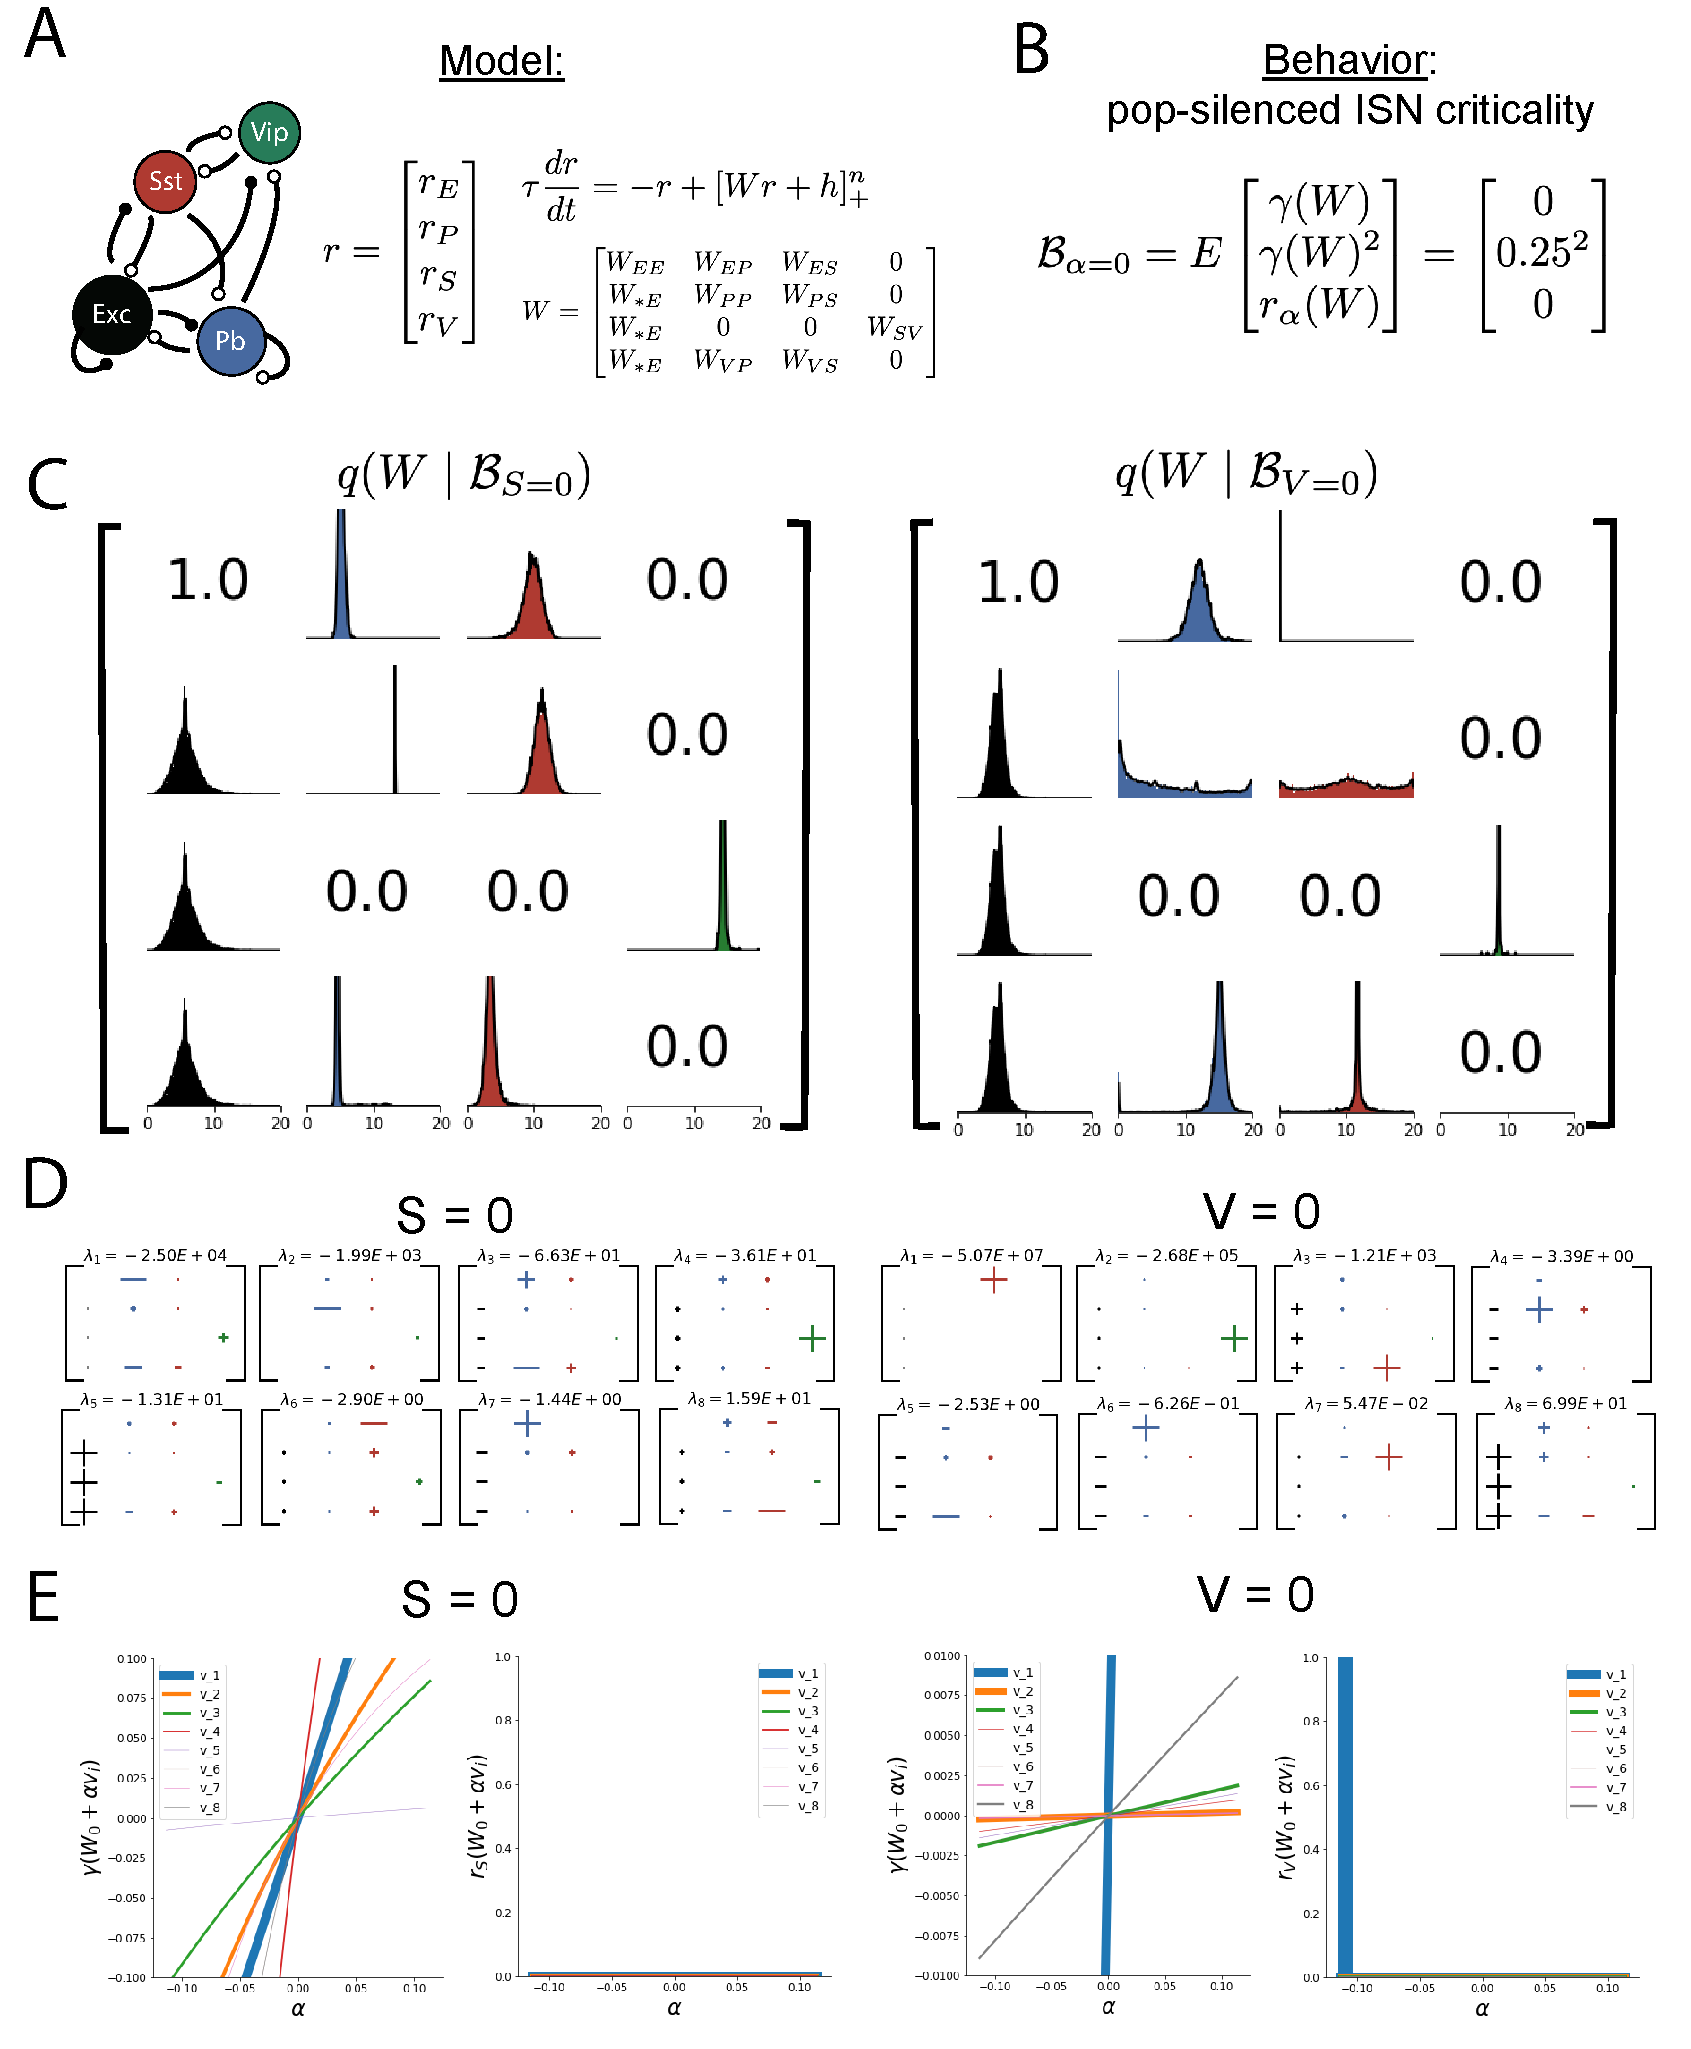
\includegraphics[scale=0.4]{V1_Fig/V1_Fig.pdf}

\caption{\footnotesize \protectA.) Model of primary visual cortex (V1) Neurons: E (black), P (blue), S (red), and V (green).  Parameters: weights of the dynamics matrix $W$.  B.) The DSNs are conditioned on population-silenced ISN criticality.  C.) DSN distribution of the parameters of the V1 model conditioned on population-silened ISN criticality.  D.) Eigenmodes of the hessian of each DSN ordered by eigenvalue.  E. Input to silenced population across ISN regimes of the DSN posterior.
}
\end{center}
\vspace{-1.cm}
\end{wrapfigure}
\small
Dynamical models with two populations (excitatory (E) and inhibitory (I) neurons) of visual processing have been used to reproduce a host of experimentally documented phenomena in V1.   When an inhibition stabilized network (ISN, the I population stabilizes an otherwise unstable E population), these models exhibit the paradoxical effect \cite{tsodyks1997paradoxical}, selective amplification \cite{murphy2009balanced}, surround suppression \cite{ozeki2009inhibitory}, and  sensory integrative properties \cite{rubin2015stabilized}.  Since I neurons mostly fall into one of three classes (parvalbumin (P)-, somatostatin (S)-, and vasointestinal peptide (V)-expressing neurons) \cite{markram2004interneurons, rudy2011three}, theorists look to extend these dynamical models to four populations \cite{litwin2016inhibitory}.  A current challenge in theoretical neuroscience is understanding the distributed role of inhibition stabilization across these subtypes.  

These four populations exhibit neuron-type specific connectivity (Fig. 1A) \cite{pfeffer2013inhibition}, in which some populations do not project to others.  Since S and V are the only populations that mutually inhibit each other, a popular conceptualization is that S and V have winner-take-all dynamics.  In fact, evidence in mice suggests that V silences S when presented with large stimuli, and S silences V for small stimuli \cite{dipoppa2018vision}.  Here, we use DSNs to understand the possible sources of inhibition stabilization in this V1 model, when either S or V is inactive.  The behavior of the DSN distributed models are constrained to produce two things: 1.) a mean-zero distribution of ISN coefficients $\gamma(W) = 1 - f^{'}(f^{-1}(r_E(W)))W_{EE}$ with some variance, and 2.) $\alpha$-population silencing $r_\alpha(W) = 0$, for $\alpha \in \{ S, V \}$ (Fig. 1B).  When $\gamma < 0$ the network is ISN, and not ISN otherwise.  Constraining the DSN behavior to a zero-mean distribution of ISN coefficients gives us samples of both ISN and non-ISN networks, optimizied to have greatest variety of stabilization motifs.

When optimized to produce a variety of stabilization motifs, there are informative differences between S-silenced and V-silenced DSN posteriors.  The marginal posteriors for each weight matrix element ($W_{EE}$ is fixed to 1.0, and $W_{*E}$ is one parameter), are visualized by their location in the dynamics matrix (Fig. 1C).  Low-variance marginals, like $q_\theta(W_{PP} \mid \mathcal{B}_{S=0})$, $q_\theta(W_{VP} \mid \mathcal{B}_{S=0})$, and $q_\theta(W_{SV} \mid \mathcal{B}_{S=0})$, indicate that either the $\gamma(W)$, S-silencing, or both are sensitive to changes in such parameters.  Whereas, $q_\theta(W_{PP} \mid \mathcal{B}_{V=0})$ and $q_\theta(W_{PS} \mid \mathcal{B}_{V=0})$ have high variance indicating degeneracy with respect to $\gamma(W)$ and V-silencing. 

As with the STG circuit, we evaluate the Hessian of the DSN posterior at $\gamma(W)=0$, and visualize the eigendecompositions ordered by eigenvalues (Fig. 1D).  In accordance with the marginals, $W_{PP}$, $W_{VP}$, and $W_{SV}$ are pronounced in the Hessian eigenvectors with the greatest magnitude eigenvalues.  The low magnitude eigenvalues indicate degenerate  dimensions of the weight matrix w.r.t. $\mathcal{B}_{\alpha=0}$.

Having a distribution optimized to be as random as possible allows us to see the variety of way in which populations are silenced across ISN regimes.  We show how E- and V-input to a silenced S population and P- and S- input to a silenced V population change with ISN regime (Fig. 1E).







\clearpage

\bibliography{v1}
\bibliographystyle{unsrt}

\end{document}

